\documentclass[11pt]{exam}
\usepackage[a4paper,width=170mm,top=20mm,bottom=25mm]{geometry}
%\usepackage[top=1in, bottom=1.25in, left=1.25in, right=1.25in]{geometry}
\usepackage{graphicx,lastpage}
\usepackage{upgreek}
\usepackage{censor}
\usepackage{tabularx}
\usepackage{xcolor}
\usepackage{amsmath}
%\usepackage{cleveref}
%\usepackage{tabularx,pbox}
%\usepackage[nopar]{lipsum}
\usepackage{longtable}
\usepackage{multirow}
\usepackage[inline]{enumitem}
\usepackage{float}
%\usepackage{tikz}
\usepackage{amssymb}
\usepackage{pdfrender}
\usepackage{pgfplots}  
\pgfplotsset{width=10cm,compat=1.8} 
\newcommand*{\boldcheckmark}{%
	\textpdfrender{
		TextRenderingMode=FillStroke,
		LineWidth=.5pt, % half of the line width is outside the normal glyph
	}{\checkmark}%
}
\setlength{\parindent}{0pt}
\definecolor{blue(pigment)}{rgb}{0.2, 0.2, 0.6}
\flushbottom
\usepackage[normalem]{ulem}
\renewcommand{\thesection}{\large \Roman{section}}
\pagestyle{headandfoot}
\usepackage{dcolumn}
\usepackage{colortbl}

\begin{document}

%==============================================================
	\begin{minipage}{\linewidth}
	\begin{minipage}{0.14\linewidth}%
		
\includegraphics[width=0.85\textwidth]{iare.png}\end{minipage}
	\begin{minipage}[r]{0.86\textwidth}%
		\noindent
		\begin{center}	
			\renewcommand{\arraystretch}{1.0}
			\textcolor{blue}{\Large \bfseries INSTITUTE OF AERONAUTICAL ENGINEERING}\\
			%\hspace*{5.2cm} 
			\textcolor{blue}{\Large (Autonomous)} \\
			%\hspace*{4.7cm}
			\small Dundigal, Hyderabad - 500 043 \\  [3pt] 
			\large \bfseries AERONAUTICAL ENGINEERING \\\vspace{2pt}
	\textcolor{red}{\large \bfseries COURSE DESCRIPTION} \\\vspace{3pt}
\end{center}
\end{minipage}\end{minipage}
\par
\newcolumntype{C}[1]{>{\centering\arraybackslash}p{#1}}
\newcolumntype{R}[1]{>{\raggedright\arraybackslash}p{#1}}
\renewcommand{\arraystretch}{1.2}
%\vspace{0.5cm}
\begin{flushleft}
	\begin{tabular}{|>{\raggedright\arraybackslash}p{4.3cm}  | >{\centering\arraybackslash}p{2.2cm}  |   >{\centering\arraybackslash}p{2.2cm} |>{\centering\arraybackslash}p{2.2cm}|>{\centering\arraybackslash}p{2.2cm}  | >{\centering\arraybackslash}p{2cm}  |   }
	\hline
		Course Title                      & \multicolumn{5}{l|}{Flight simulation and Controls Laboratory \textbf{\begin{tabular}[l]{@{}l@{}} \end{tabular}}}                                                                  \\ \hline
	Course Code                       & \multicolumn{5}{l|}{BAED23}                                                                              \\ \hline
	Program                           & \multicolumn{5}{l|}{M.Tech}                                                                              \\ \hline
	Semester                          & \multicolumn{5}{l|}{II}                                            \\ \hline
	Course Type                       & \multicolumn{5}{l|}{ Laboratory }          \\ \hline
	Regulation                        & \multicolumn{5}{l|}{MT-23}     \\ \hline
	\multirow{3}{*}{Course Structure} & \multicolumn{3}{c|}{Theory}                                             & \multicolumn{2}{c|}{Practical} \\ \cline{2-6} 
	& \multicolumn{1}{c|}{Lecture} & \multicolumn{1}{c|}{Tutorials} & Credits & Laboratory      & Credits      \\ \cline{2-6} 
	& \multicolumn{1}{c|}{-}       & -                              & -       & 3              & 1.5         \\ \hline
	Course Coordinator                 & \multicolumn{5}{l|}{Mr. K Arun Kumar,  Assistant Professor}                                          \\ \hline
\end{tabular}
\end{flushleft}
\vspace{-0.5cm}
\begin{flushleft}
	\textcolor{blue}{\section{\large \bfseries COURSE PRE-REQUISITES:}}\vspace{-0.2cm}
	\begin{tabular}{|>{\centering\arraybackslash}p{3cm}  | >{\centering\arraybackslash}p{4cm}  |   >{\centering\arraybackslash}p{3cm} |>{\centering\arraybackslash}p{5cm}|} 
		\hline 		
		\textbf{Level}&	\textbf{Course Code}&	\textbf{Semester}&	\textbf{Prerequisites}\\ 
		\hline
	B.Tech&	AAED08&	IV&	Aerodynamics\\ \hline
	B.Tech&	AAEC16&	V&	High Speed Aerodynamics\\ \hline
	B.Tech&	AAED25&	VI&	Computational Aerodynamics\\ \hline
\end{tabular}\end{flushleft}
\textcolor{blue}{\section{\large \bfseries COURSE OVERVIEW:}}
Flight simulation and Control is the science that investigates the stability and control of aircrafts and all other flying vehicles. From the advent of the first flight by the Wright Brothers, it was observed that flight without knowledge of stability and control was not viable. Since then, several different concepts for controlling aircraft flight have been devised including control surfaces, deformable surfaces, morphing of wings etc. This course introduces some of these concepts and describes their operation, as well as the degree of stability that these devices can provide. Modern aircraft control is ensured through automatic control systems known as autopilot. Their role is to increase safety, facilitate the pilot's task and improve flight qualities. The course will introduce modern aircraft stability and control and discuss some of its objectives and applications
\begin{flushleft}\vspace{-0.75cm}
\textcolor{blue}{\section{\large \bfseries MARKS DISTRIBUTION:}}\vspace{-0.2cm}
	\begin{tabular}{|>{\centering\arraybackslash}p{5cm}  | >{\centering\arraybackslash}p{3.75cm}  |   >{\centering\arraybackslash}p{3.75cm} |>{\centering\arraybackslash}p{2.8cm}|}
		\hline 
	\textbf{Subject}&	\textbf{SEE Examination}&	\textbf{CIE Examination}&	\textbf{Total Marks}\\ 
	\hline
Flight simulation and Controls Laboratory	&	70 Marks&	30 Marks&	100\\ 
	\hline
	\end{tabular}
\end{flushleft}\vspace{-1cm}
\begin{flushleft}
\textcolor{blue}{\section{\large \bfseries DELIVERY / INSTRUCTIONAL METHODOLOGIES:}}\vspace{-0.2cm}
	\begin{tabular}{|>{\centering\arraybackslash}p{0.3cm}  | >{\centering\arraybackslash}p{2.3cm}  |   >{\centering\arraybackslash}p{0.5cm} |>{\centering\arraybackslash}p{2.4cm}|>{\centering\arraybackslash}p{0.5cm}  | >{\centering\arraybackslash}p{3cm}  |   >{\centering\arraybackslash}p{0.5cm} |>{\centering\arraybackslash}p{4cm}|}
	\hline 

\checkmark &  Demo Video  & \checkmark& Lab Worksheets &  \checkmark & Viva Questions  & \checkmark &  Probing further Questions \\ \hline
\end{tabular}
\end{flushleft}
\vspace{-2.5cm}
\newpage
\textcolor{blue}{\section{\large \bfseries EVALUATION METHODOLOGY:}}\vspace{-0.2cm}
Each lab will be evaluated for a total of 100 marks consisting of 30 marks for internal assessment and 70
marks for semester end lab examination. Out of 30 marks of internal assessment, continuous lab
assessment will be done for 20 marks for the day to day performance and 10 marks for the final internal
lab assessment. The semester end lab examination for 70 marks shall be conducted by two examiners, one
of them being a internal examiner and another is external examiner, both nominated by the Principal from
the panel of experts recommended by Chairman, BOS.

All the drawing related courses are evaluated in line with lab courses. The distribution shall be 30 marks
for internal evaluation (20 marks for day–to–day work, and 10 marks for internal tests) and 70 marks for
semester end lab examination. There shall be ONE internal test for 10 marks each in a semester.

The emphasis on the experiments is broadly based on the following criteria given in Table: 1
\begin{longtable}{|C{4cm}|C{5.8cm}|C{5.6cm}|}
	\hline
	&Experiment Based	&	Programming based\\ \hline
20 \%&	Objective&	Purpose\\ \hline
20 \%&	Analysis&	Algorithm\\ \hline
20 \%&	Design&	Programme\\ \hline
20 \%&	Conclusion&	Conclusion\\ \hline
20 \%&	Viva&	Viva\\ \hline
\end{longtable}
\textcolor{blue}{\textbf{\large  Continuous Internal Assessment (CIA):}}\\
CIA is conducted for a total of 30 marks (Table 1), with 20 marks for continuous lab assessment during day to day performance, 10 marks for final internal lab assessment. 
\begin{longtable}{|C{2.5cm}|C{4.3cm}|C{4.5cm}|C{3.5cm}|}
	\hline
\centering \textbf{Component}&	\multicolumn{2}{c|}{\textbf{Laboratory}}    &	 \multirow{2}{*}{\textbf{Total Marks}} \\ \cline{1-3}
\textbf{Type of Assessment}&	\textbf{Day to day performance}&	\textbf{Final internal lab assessment}&	\\\hline
CIA Marks&	20&	10&	30\\\hline
\end{longtable}
\textcolor{blue}{\textbf{\large Continuous Internal Examination (CIE):}}\\
One CIE exams shall be conducted at the end of the 16th week of the semester. The CIE exam is conducted for 10 marks of 3 hours duration.\\
\begin{enumerate}
	\item \textbf{Experiment Based }
\begin{longtable}{|C{2.2cm}|C{2.2cm}|C{2.2cm}|C{2.42cm}|C{2.42cm}|C{2.2cm}|}
	\hline
Objective&	Analysis&	Design&	Conclusion&	Viva&	Total\\\hline
2&	2&	2&	2&	2&	10\\\hline
\end{longtable}
\item \textbf{Programming Based }
\begin{longtable}{|C{2.2cm}|C{2.2cm}|C{2.2cm}|C{2.42cm}|C{2.42cm}|C{2.2cm}|}
	\hline
	Objective&	Analysis&	Design&	Conclusion&	Viva&	Total\\\hline
	2&	2&	2&	2&	2&	10\\\hline
\end{longtable}
\end{enumerate}\vspace{-1cm}
\newpage
\textcolor{blue}{\section{\large \bfseries COURSE OBJECTIVES:}}\vspace{-0.4cm}

%	\flushleft\textbf{\textcolor{blue}{\large COURSE OBJECTIVES:}}\\		
\textbf{The students will try to learn:}\vspace{-0.4cm}
\newcolumntype{C}[1]{>{\centering\arraybackslash}p{#1}}
\newcolumntype{R}[1]{>{\raggedright\arraybackslash}p{#1}}
\renewcommand{\arraystretch}{1.2}
\begin{flushleft}	
	\begin{longtable}{|C{1.5cm}|R{15cm}|}
		\hline
		I & The utilization of MATLAB-SIMULINK and Flight-Simulator software to obtain the
		solution for complex and simple performance parametric conditions.\tabularnewline
	\hline
	II & The involvement of various mathematical conditions. \tabularnewline
	\hline
	III &  The complex performance by using MATLAB-Simulator to determine the flight
	performance and stability criteria.\tabularnewline
	\hline	
	\end{longtable}
\end{flushleft}\vspace{-2cm}
\textcolor{blue}{\section{\large \bfseries COURSE OUTCOMES:}}\vspace{-0.4cm}
\textbf{After successful completion of the course, students should be able to:}
\renewcommand{\arraystretch}{1.1}\vspace{-0.4cm}
\begin{flushleft}
	\begin{longtable}{|C{1.2cm}|R{13cm}|C{2cm}|}
		\hline
	
		CO 1&	\textbf{Apply } \textcolor{blue}{the philosophy behind the flight performance and condition} \textcolor{red}{for recognizing the impacting
			parameters.}   	& Apply \tabularnewline\hline
		CO 2&	\textbf{Evaluate} \textcolor{blue}{the optimized condition} \textcolor{red}{ for best performance.} 	& Evaluate \tabularnewline
		\hline  
			CO 3&	\textbf{Identify} \textcolor{blue}{the appropriate conditions} \textcolor{red}{for attaining the precise results aerospace vehicle} 	& Remember\tabularnewline\hline
		CO 4&	\textbf{Choose} \textcolor{blue}{the suitable numerical techniques and provide the economical solutions} \textcolor{red}{by using
			FLIGHT-SIMULATOR and MATLAB-SIMULINK.}	   & Apply \tabularnewline
		\hline    
			CO 5&	\textbf{Analyze} \textcolor{blue}{mission critical problems} \textcolor{red}{using MATLAB/SIMULINK Software’s and FLIGHT
				SIMULATOR.} 	& Anlayze \tabularnewline\hline
			 
		CO 6&	\textbf{Make use of} \textcolor{blue}{MATLAB/SIMULINK Software’s and FLIGHT SIMULATOR} \textcolor{red}{for assessing flight performance in given condition.}  	&Apply \tabularnewline
		\hline  
	\end{longtable}
\end{flushleft}
\textbf{\textcolor{blue}{\large COURSE KNOWLEDGE COMPETENCY LEVEL}}
\begin{center}	
	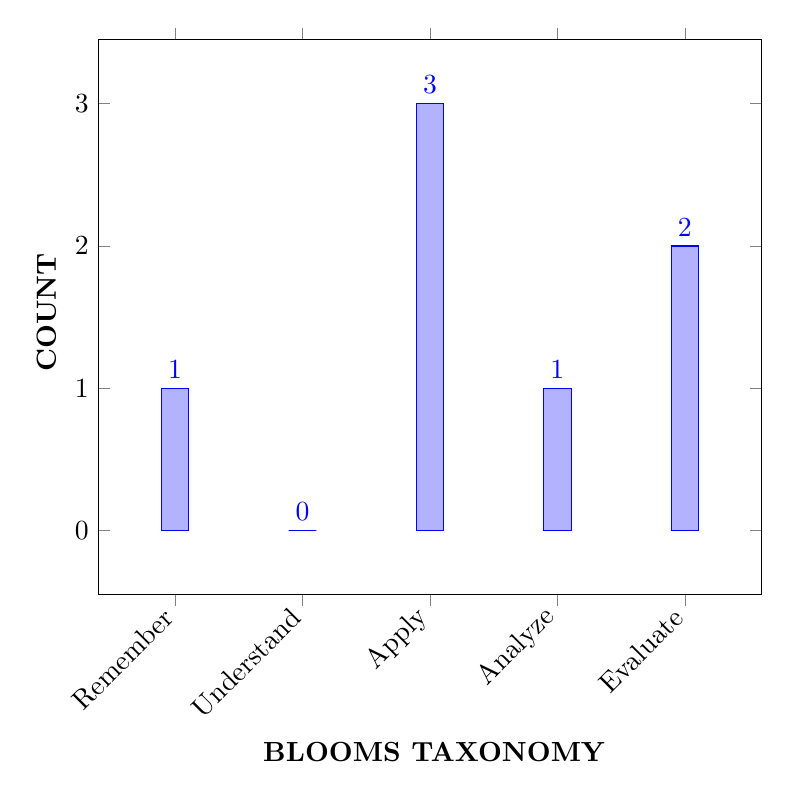
\begin{tikzpicture}  
		\begin{axis}  [
			ybar,
			enlargelimits=0.15,
			legend style={at={(0.5,-0.2)},
				anchor=north,legend columns=-1},
			ylabel={\ \textbf{COUNT} },
			xlabel={\ \textbf{BLOOMS TAXONOMY}},
			symbolic x coords={Remember,Understand,Apply,%
				Analyze,Evaluate},
			xtick=data,
			nodes near coords,
			nodes near coords align={vertical},
			x tick label style={rotate=45,anchor=east},
			]
			\addplot coordinates {
			(Remember,1) (Understand,0) (Apply,3)
			(Analyze,1) (Evaluate,2)
			};
		\end{axis}  
	\end{tikzpicture}
\end{center}
\newpage
\textcolor{blue}{\section{\large \bfseries  PROGRAM OUTCOMES: }}\vspace{-0.6cm}
\begin{flushleft}
	\begin{longtable}{|>{\centering\arraybackslash}p{1.6cm}  | >{\raggedright\arraybackslash}p{15cm}  | }
		\hline
		\multicolumn{2}{|c|}{\textbf{Program Outcomes}}  \\ \hline
		\endhead
		\hline
		PO 1&	Identify, formulate, analyze and Design complex engineering problems, and design system components or processes by applying appropriate
	advanced principles of engineering activities and using modern tools\\ \hline
	PO 2&	Engage in life-long learning and professional development through self-study
	and continuing education in understanding the engineering solutions in global and management principles to manage projects in multidisciplinary
	environments. \\ \hline
	PO 3&	Demonstrate a degree of mastery in emerging areas of Aerospace Engineering such as Aerodynamics, Propulsion, Structure and Flight
	Dynamics \\ \hline
	PO 4&	Write and present a substantial technical report/document \\ \hline
	PO 5&	Independently carry out research/investigation and development work to
	solve practical problems \\ \hline
	
	PO 6& Function effectively as a member or leader in diverse teams to carry out development work, produce solutions that meet the specified needs with
	frontier technologies and communicate effectively on complex engineering	activities. \\ \hline
	
	\end{longtable}
\end{flushleft}\
\vspace{-2cm}
%\vspace{-0.5cm}
\textcolor{blue}{\section{\large \bfseries HOW PROGRAM OUTCOMES ARE ASSESSED:}}\vspace{-0.4cm}
\begin{flushleft}
	\begin{longtable}{|>{\centering\arraybackslash}p{1.6cm}  | >{\raggedright\arraybackslash}p{8.8cm}  |   >{\centering\arraybackslash}p{1.8cm} |>{\centering\arraybackslash}p{2.7cm}|}
		\hline
		\multicolumn{2}{|c|}{\textbf{Program}} & \textbf{Strength} & \textbf{Proficiency Assessed by} \\ \hline
	PO1 &Identify, formulate, analyze and Design complex engineering problems, and design system components or processes by applying appropriate
	advanced principles of engineering activities and using modern tools	&2	&CIE, SEE	\\ \hline
	PO3 &Demonstrate a degree of mastery in emerging areas of Aerospace Engineering such as Aerodynamics, Propulsion, Structure and Flight Dynamics	&2	&CIE, SEE	\\ \hline
		PO4 &Write and present a substantial technical report/document&1	&CIE, SEE	\\ \hline
	
	PO 5&Independently carry out research/investigation and development work to
	solve practical problems	& 2	& CIE, SEE	\\ \hline


	\multicolumn{4}{l}{\textbf{3 = High; 2 = Medium; 1 = Low}}\\ 
			\end{longtable}
	\end{flushleft}

\vspace{-1.5cm}
\textcolor{blue}{\section{\large \bfseries	MAPPING COURSE OUTCOMES LEADING TO THE ACHIEVEMENT OF PROGRAM OUTCOMES AND PROGRAM SPECIFIC OUTCOMES}}\vspace{-0.4cm}
\begin{flushleft}
	\begin{longtable}{|>{\centering\arraybackslash}p{3cm}  | >{\centering\arraybackslash}p{1.75cm}  |   >{\centering\arraybackslash}p{1.75cm} |>{\centering\arraybackslash}p{1.75cm}|>{\centering\arraybackslash}p{1.75cm}  |> {\centering\arraybackslash}p{1.75cm}  |> {\centering\arraybackslash}p{1.75cm} |  }
	\hline	
\multirow{2}{*}{\textbf{\begin{tabular}[c]{@{}c@{}}\small  COURSE \\\small OUTCOMES\end{tabular}}} & \multicolumn{6}{l|}{PROGRAM OUTCOMES}  \\ \cline{2-7} 
	       &     PO 1    &   PO 2    &   PO 3     & PO 4 & PO 5 & PO 6    \\ \hline
CO 1	&    2   &  -   &   2    &1 &2 & -\\ \hline
CO 2	&  2    &  -     &  2     &1 & 2&-\\ \hline
CO 3	&   2  &   -   &    2   & 1&2 & - \\ \hline
CO 4	&  2    &  -     &  2    & 1&2 &- \\ \hline
CO 5	&  2    &  -   &  2    & 1&2 & -\\ \hline
CO 6	&   2   &  -   &  2     &1 &2 & -\\ \hline

	\end{longtable}
\end{flushleft}\vspace{-1.75cm}
\textcolor{blue}{\section{\large \bfseries ASSESSMENT METHODOLOGY DIRECT:}}\vspace{-0.24cm}

\begin{flushleft}	
	\begin{tabular}{|>{\centering\arraybackslash}p{3cm}  | >{\centering\arraybackslash}p{2.2cm}  |   >{\centering\arraybackslash}p{3cm} |>{\centering\arraybackslash}p{2.5cm}|>{\centering\arraybackslash}p{2.6cm}  |>{\centering\arraybackslash}p{1cm}  | } 
		\hline 		
	CIE Exams            & \checkmark & SEE Exams       & \checkmark & Seminars               & -     \\ \hline
	Laboratory Practices &     \checkmark               & Student Viva    &       \checkmark          & Certification          & - \\ \hline

	\end{tabular}
\end{flushleft}
\vspace{-1cm}
\textcolor{blue}{\section{\large \bfseries	ASSESSMENT METHODOLOGY INDIRECT:}}\vspace{-0.5cm}	
	\begin{longtable}{|C{1.2cm}|R{6cm}|C{1.3cm}|R{6.5cm}|}
		\hline
	\boldcheckmark&	Early Semester Feedback&	\boldcheckmark &	End Semester OBE Feedback\\\hline
	\textbf{X}&	\multicolumn{3}{l|}{Assessment of Mini Projects by Experts} \\\hline
\end{longtable}
\vspace{-1cm}
\textcolor{blue}{\section{\large \bfseries	SYLLABUS:}}	\vspace{-0.4cm}
  
	\centering
	\renewcommand{\arraystretch}{1.2}
\begin{longtable}{|>{\centering\arraybackslash}p{2cm}  | >{\raggedright\arraybackslash}p{14cm}  | }
		\hline 
		WEEK I & \textcolor{blue}{\textbf{SIMULATION OF UNACCELERATED AND ACCELERATED LEVEL FLIGHT}}\\
	\hline
	& Implement the following tasks
	\begin{enumerate}
		\item Simulation of steady flight.
		\item Simulation of accelerated level flight at various altitudes.
	\end{enumerate}
 \\\hline
	WEEK II & \textcolor{blue}{\textbf{SIMULATION OF UNACCELERATED AND ACCELERATED CLIMB}}\\
	\hline
	& Implement the following tasks
		\begin{enumerate}
	\item  Simulation of steady climb
	\item Simulation of accelerated climb at various climb rates 
\end{enumerate}\\	\hline
	WEEK III & \textcolor{blue}{\textbf{SIMULATION OF UNACCELERATED AND ACCELERATED DESCENT}}\\
	\hline
	& Implement the following tasks
	\begin{enumerate}
		\item Simulation of steady descent
	\item Simulation of accelerated descent at various descentrates
\end{enumerate}
	 \\
	\hline
	WEEK IV & \textcolor{blue}{\textbf{SIMULATION OF TAKE-OFF PERFORMANCE}}\\
	\hline
	& Implement the following tasks 
	\begin{enumerate}
		\item Estimation of take off velocity for Cessna flight.
	\end{enumerate}
		\\
	\hline
	WEEK V & \textcolor{blue}{\textbf{SIMULATION OF LANDING PERFORMANCE}}\\
	\hline
	& Implement the following tasks
	\begin{enumerate}
	\item Estimation of ground roll distance for Cessna flight
	\item Estimation of total landing distance for Cessna flight 
		\end{enumerate} \\
	\hline
	WEEK VI & \textcolor{blue}{\textbf{SIMULATION OF CONVENTIONAL FLIGHT PATH}}\\
	\hline
	& Implement the following tasks 
	\begin{enumerate}
	 \item Perform the given mission profiles
	\end{enumerate}
\\
	\hline
	WEEK VII & \textcolor{blue}{\textbf{STABILIZATION OF LONGITUDINAL PER TURBED AIRCRAFT}}\\
	\hline
	&Implement the following tasks
	\begin{enumerate}
\item Perform the operation from disturbed flight to trim flight
\item Perform long period and short period modes. 
		\end{enumerate}\\
	\hline
	WEEK VIII & \textcolor{blue}{\textbf{STABILIZATION OF LATERAL PERTURBED AIRCRAFT}}\\
	\hline
	&Implement the following tasks
	\begin{enumerate}
\item  Perform the operation from disturbed flight to trim flight
	\item Simulate lateral directional modes.
\end{enumerate} \\
	\hline
	WEEK IX & \textcolor{blue}{\textbf{SIMULATION OF SPIN RECOVERY}}\\
	\hline
	&Implement the following tasks 
	\begin{enumerate}
	\item  Perform the operation of spin recovery
\end{enumerate}	\\
	\hline
	
	WEEK X & \textcolor{blue}{\textbf{SIMUILATION OF COORDINATED LEVEL TURN}}\\
	\hline
	&Implement the following tasks
\begin{enumerate}
	\item Perform the level turn at given turn rate.
\item Perform the level turn at given turn radius.
\end{enumerate}	
	\\
	\hline
	WEEK XI & \textcolor{blue}{\textbf{SIMUILATION OF BARREL ROLL MANEUVER}}\\
	\hline
	& Implement the following tasks 
	\begin{enumerate}
	\item Perform the barrel roll maneuver
\end{enumerate}	
	\\
	\hline
	WEEK XII & \textcolor{blue}{\textbf{SIMULATION OF A COMPLEX FLIGHT PATH}}\\
	\hline
	&Implement the following tasks
	\begin{enumerate}
	\item Perform flight simulation for given mission profiles
\end{enumerate}	
	\\
	\hline
	
\end{longtable}
%\newpage
\raggedright	\textcolor{blue}{\textbf{TEXTBOOKS}}\\
\begin{enumerate}
	\item	Peter John Davison, ―A summary of studies conducted on the effect of motion in flight simulator pilot training", 5th February, 2014.


\end{enumerate}
	
  \textcolor{blue}{\textbf{REFERENCE BOOKS:}}\\
\begin{enumerate}
	\vspace{-0.5cm}
	\item Vepa, R., ―Flight Dynamics, Simulation and Control: For Rigid and Flexible Aircraft‖, CRC Press, Taylor and Francis Group, 2015.
\item Wayne Durham, ―Aircraft Flight Dynamics and Control‖, CRC Press, 2nd Edition, 2013.
\item RobertF.Stengel ―Flight Dynamics‖, CRC Press, 2nd Edition, 2013.
\end{enumerate}
\newpage
\vspace{-1cm} 
\textcolor{blue}{\section{\large \bfseries	COURSE PLAN:}}\vspace{-0.4cm}
The course plan is meant as a guideline. Probably there may be changes.

\begin{flushleft}
	\begin{longtable}{|>{\centering\arraybackslash}p{1cm}  | >{\raggedright\arraybackslash}p{7cm}  |   >{\centering\arraybackslash}p{5cm} |>{\centering\arraybackslash}p{1.8cm}|}
		\hline 
			\textbf{S.No}&	\centering{\textbf{ Topics to be covered}} &	\textbf{CO's}&\textbf{Reference}\\ 
		\hline
1&	\lowercase{SIMULATION OF UNACCELERATED AND ACCELERATED LEVEL FLIGHT} &	CO 1&	T1: 2.3\\
\hline
2&\lowercase{SIMULATION OF UNACCELERATED AND ACCELERATED CLIMB} &	CO 1&	T1: 2.6\\
\hline
3&	\lowercase{SIMULATION OF UNACCELERATED AND ACCELERATED DESCENT}	& CO 1&	T1: 2.6\\
\hline
4&	\lowercase{SIMULATION OF TAKE-OFF PERFORMANCE}&	CO 2 &	T1: 2.7
\\
\hline
5&	\lowercase{SIMULATION OF LANDING PERFORMANCE}& CO 2	&	R1: 2.22\\
\hline
6&	\lowercase{SIMULATION OF CONVENTIONAL FLIGHT PATH}& CO 3 &	R1: 2.25\\
\hline
7&	\lowercase{STABILIZATION OF LONGITUDINAL PERTURBED AIRCRAFT} & CO 4& R1: 2.55
\\
\hline
8&	\lowercase{STABILIZATION OF LATERAL PERTURBED AIRCRAFT} & CO 4&	R1: 2.3\\
\hline
9&	\lowercase{SIMULATION OF SPIN RECOVERY} &CO 5&	R1: 2.6\\
\hline
10&	\lowercase{SIMULATION OF COORDINATED LEVEL TURN} &	CO 6&	R1: 2.8\\
\hline
11&	\lowercase{SIMULATION OF BARREL ROLL MANEUVER} &	CO 6 &	
R1:2.18\\
\hline
12&	\lowercase{SIMULATION OF A COMPLEX FLIGHT PATH}& CO 3 &	R3:5.22\\
\hline
	\end{longtable}
	\vspace{-1cm}
\end{flushleft}
\textcolor{blue}{\section{\large \bfseries	EXPERIMENTS FOR ENHANCED LEARNING (EEL):}}\vspace{-0.6cm}
	\begin{longtable}{|>{\centering\arraybackslash}p{1cm}  | >{\raggedright\arraybackslash}p{15cm}  |   }
	\hline
\textbf{S.No}&\textbf{\centering Design Oriented Experiments} \\
	\hline
	1&	Simulation of Acclerated and unacclerated flight during various flight conditions
\\
\hline
2&	Simulation of landing and take off performance of  Cessna 172 Skyhawk
\\
\hline
3&	
Simulation of Low level strike profile\\
\hline
4&	
Simulation of hall roll, split S and Loop profile flight \\
\hline
5&	
Simulation of cobra maneuvering \\
\hline
\end{longtable}
\vspace{2cm}
\flushleft \textbf{Signature of Course Coordinator}\hspace{8cm} \textbf{HOD, AE}\\\textbf{Mr. K Arun Kumar,  Assistant Professor}\\


\end{document}
}